\begin{frame}
    \frametitle{Transformaciones en 2D}
    \small
    \begin{center}
        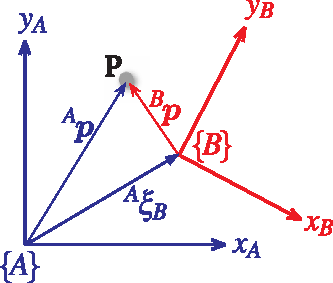
\includegraphics[width=0.3\columnwidth]{./images/coordinate_frames.pdf}
    \end{center}


    El punto $\point$ puede describirse mediante vectores de coordenadas relativos a cualquier marco $\{\mathrm{A}\}$ o $\{\mathrm{B}\}$. La pose de $\{\mathrm{B}\}$ relativa a $\{\mathrm{A}\}$ es $\transform{A}{B}$.
    \begin{align*}
        \pointCoord{A} &= \transform{A}{B}\pointCoord{B}\\
        \transform{A}{C} &= \transform{A}{B}\transform{B}{C}\\
        \transform{A}{B} &= \transform{B}{A}^{-1}
    \end{align*}

\end{frame}


\begin{frame}
    \frametitle{Transformaciones en 2D}
    
    \begin{figure}[!h]
        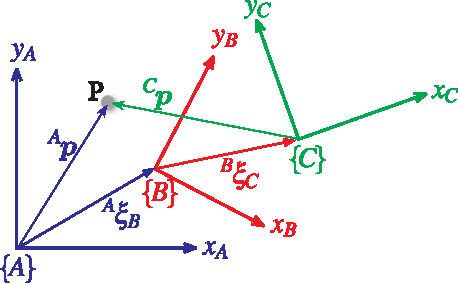
\includegraphics[width=0.6\columnwidth]{./images/multiple_coordinate_frames_2d.pdf}
    \end{figure}

\end{frame}


\begin{frame}
    \frametitle{Transformaciones en 3D}

    \begin{figure}[!h]
        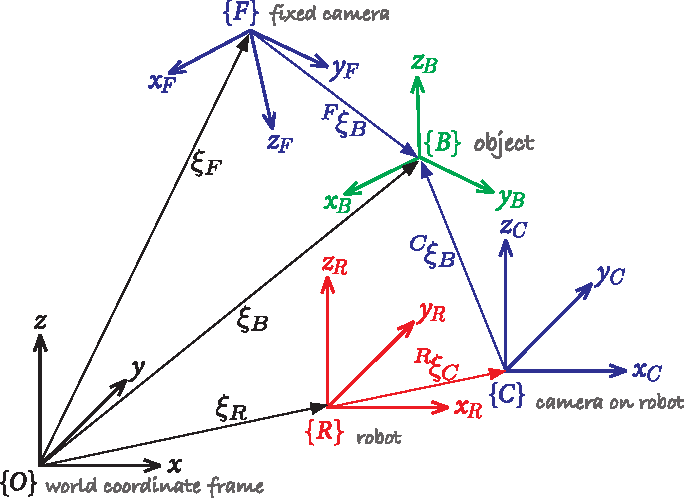
\includegraphics[width=0.6\columnwidth]{./images/multiple_coordinate_frames_3d.pdf}
    \end{figure}

\end{frame}

\begin{frame}
    \frametitle{Transformaciones...}
    
    \begin{figure}[!h]
        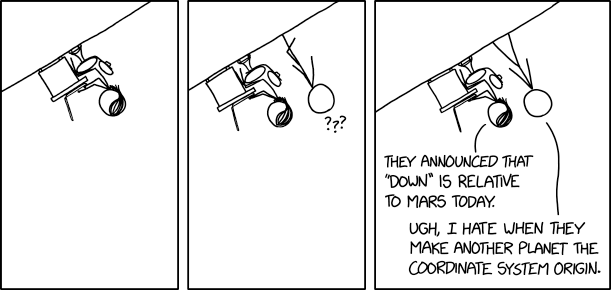
\includegraphics[width=\columnwidth]{./images/joke_coordinate_systems.png}
    \end{figure}
    
\end{frame}


\begin{frame}
    \frametitle{Rotación en 2D}

        \begin{center}
        \begin{minipage}{0.4\linewidth}
            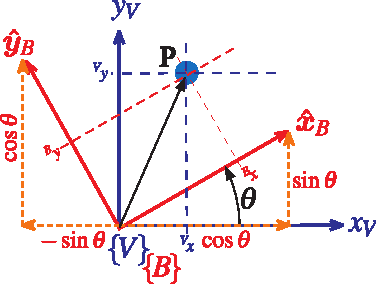
\includegraphics[width=\columnwidth]{coordinate_system_rotation.pdf}
        \end{minipage}
        \hspace{1em}
        \begin{minipage}{0.5\linewidth}
            \begin{equation*}
                R(\theta) =
                \toCoord{\fromCoord{\begin{bmatrix}
                    \cos \theta & -\sin \theta \\
                    \sin \theta & \cos \theta
                \end{bmatrix}}{A}}{B}
            \end{equation*}

            \begin{equation*}
                \begin{bmatrix}
                    \toCoord{x}{B}\\
                    \toCoord{y}{B}
                \end{bmatrix} =
                \toCoord{\fromCoord{\begin{bmatrix}
                    \cos \theta &-\sin \theta \\
                    \sin \theta &\cos \theta
                \end{bmatrix}}{A}}{B}
                \begin{bmatrix}
                    \toCoord{x}{A}\\
                    \toCoord{y}{A}
                \end{bmatrix}
            \end{equation*}

            \begin{align*}
                \toCoord{x}{B} &= \toCoord{x}{A} \cos \theta -\toCoord{y}{A} \sin \theta\\
                \toCoord{y}{B} &= \toCoord{x}{A} \sin \theta + \toCoord{y}{A}\cos \theta
            \end{align*}

            \begin{equation*}
                \begin{bmatrix}
                    \toCoord{x}{B}\\
                    \toCoord{y}{B}
                \end{bmatrix} =
                \rotationCoord{B}{A}
                \begin{bmatrix}
                    \toCoord{x}{A}\\
                    \toCoord{y}{A}
                \end{bmatrix}
            \end{equation*}
        \end{minipage}
    \end{center}
\end{frame}


\begin{frame}
    \frametitle{Ejercicio: Rotación en 2D}
    
    \centering
    
    \begin{center}
        \begin{minipage}{0.4\linewidth}
            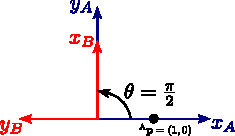
\includegraphics[width=\columnwidth]{rotation_2D_example.pdf}
        \end{minipage}
        \hspace{1em}
        \begin{minipage}{0.5\linewidth}
            
            \only<1>{
                \begin{equation*}
                    \toCoord{\point}{B} = \, ?
                \end{equation*}
            }
            \only<2>{
                \begin{equation*}
                    \toCoord{\point}{B} = \rotationCoord{B}{A} \toCoord{\point}{A}
                \end{equation*}
               
                \begin{equation*}
                    R\left(\frac{\pi}{2}\right) =
                    \toCoord{\fromCoord{\begin{bmatrix}
                        \cos \frac{\pi}{2} & -\sin \frac{\pi}{2} \\
                        \sin \frac{\pi}{2} & \cos \frac{\pi}{2}
                    \end{bmatrix}}{A}}{B} =
                    \toCoord{\fromCoord{\begin{bmatrix}
                        0 & 1 \\
                        -1 & 0
                    \end{bmatrix}}{A}}{B}
                \end{equation*}
                
                \begin{equation*}
                    \toCoord{\begin{bmatrix}
                        0\\
                        -1
                    \end{bmatrix}}{B} =
                    \toCoord{\fromCoord{\begin{bmatrix}
                        0 & 1 \\
                        -1 & 0
                    \end{bmatrix}}{A}}{B}
                    \toCoord{\begin{bmatrix}
                        1\\
                        0
                    \end{bmatrix}}{A}
                \end{equation*}                
            }
        \end{minipage}
    \end{center}
\end{frame}



\begin{frame}
    \frametitle{Rototraslación en 2D}
\scriptsize
Solo traslación:
    \begin{equation*}
        \begin{bmatrix}
            \toCoord{x}{B}\\
            \toCoord{y}{B}
        \end{bmatrix} =
        \begin{bmatrix}
            \toCoord{x}{A}\\
            \toCoord{y}{A}
        \end{bmatrix} +
        \begin{bmatrix}
            \toCoord{t_{x}}{A}\\
            \toCoord{t_{y}}{A}
        \end{bmatrix}
    \end{equation*}
Agregando Rotación:
    \begin{align*}
        \begin{bmatrix}
            \toCoord{x}{B}\\
            \toCoord{y}{B}
        \end{bmatrix} &=
       \toCoord{\fromCoord{\begin{bmatrix}
                                \cos \theta & -\sin \theta \\
                                \sin \theta & \cos \theta
                            \end{bmatrix}}{A}}{B}
        \begin{bmatrix}
            \toCoord{x}{A}\\
            \toCoord{y}{A}
        \end{bmatrix} +
        \begin{bmatrix}
            \toCoord{t_{x}}{A}\\
            \toCoord{t_{y}}{A}
        \end{bmatrix}
    \end{align*}

Representamos las matrices y vectores simbólicamente:

    \begin{equation*}
        \begin{bmatrix}
            \toCoord{x}{B}\\
            \toCoord{y}{B}\\
        \end{bmatrix} = \rotationCoord{B}{A}
        \begin{bmatrix}
            \toCoord{x}{A}\\
            \toCoord{y}{A}
        \end{bmatrix} + \toCoord{\translation}{A}
    \end{equation*}


Armamos la matriz de rototraslación, y utilizamos coordenadas homogéneas:

    \begin{align*}
        \begin{bmatrix}
            \toCoord{x}{B}\\
            \toCoord{y}{B}\\
            1
        \end{bmatrix} &=
        \begin{bmatrix}
            \rotationCoord{B}{A} & \toCoord{\translation}{A}\\
            \vec{0} & 1
        \end{bmatrix}
        \begin{bmatrix}
            \toCoord{x}{A}\\
            \toCoord{y}{A}\\
            1
        \end{bmatrix}\\
        \begin{bmatrix}
            \toCoord{x}{B}\\
            \toCoord{y}{B}\\
            1
        \end{bmatrix} &=
        \transform{B}{A}
        \begin{bmatrix}
            \toCoord{x}{A}\\
            \toCoord{y}{A}\\
            1
        \end{bmatrix}
    \end{align*}


\end{frame}


\begin{frame}
    \frametitle{Algunas Propiedades de las transformaciones}

    \begin{itemize}
        \item Composición:
        \begin{equation*}
            \transform{}{1}\transform{}{2} =
            \begin{bmatrix}
                \rotationCoord{}{1} & \translationCoord{}{1}\\
                \vec{0} & 1
            \end{bmatrix}
            \begin{bmatrix}
                \rotationCoord{}{2} & \translationCoord{}{2}\\
                \vec{0} & 1
            \end{bmatrix} =
            \begin{bmatrix}
                \rotationCoord{}{1}\rotationCoord{}{2} & \translationCoord{}{1}+\rotationCoord{}{1}\translationCoord{}{2}\\
                \vec{0} & 1
            \end{bmatrix}
        \end{equation*}
        
        \item Inversa:
        \begin{equation*}
            \transform{}{}^{-1}=
            \begin{bmatrix}
                \rotation & \translation\\
                \vec{0} & 1
            \end{bmatrix}^{-1} =
            \begin{bmatrix}
                \rotation^{\top} & -\rotation^{\top}\translation\\
                \vec{0} & 1
            \end{bmatrix}
        \end{equation*}
        
        \item $\transform{}{} \in SE(3)$
    \end{itemize}



\end{frame}


\begin{frame}
    \frametitle{Pose}
    
    La Pose (posición y orientación) de un robot es la transformación rototraslacional dada por la posición y orientación del robot en el espacio.
    
    Ejemplo: Dado el vector posición $\toCoord{\position}{\worldCoordSystem}$ y la matriz orientación $\toCoord{\fromCoord{\orientation}{\bodyCoordSystem}}{\worldCoordSystem}$ del robot $\bodyCoordSystem$ en el mundo $\worldCoordSystem$, notamos la pose como $\transform{\worldCoordSystem}{\bodyCoordSystem}$
    
    \begin{equation*}
        \transform{\worldCoordSystem}{\bodyCoordSystem}=
        \begin{bmatrix}
            \toCoord{\fromCoord{\orientation}{\bodyCoordSystem}}{\worldCoordSystem} & \toCoord{\position}{\worldCoordSystem}\\
            \vec{0} & 1
        \end{bmatrix}
    \end{equation*}

    Observar que la pose es una transformación que toma elementos en coordenadas del robot y los devuelve en coordenadas del mundo.
\end{frame}


\begin{frame}
    \frametitle{Coordenadas Homogeneas e Hinomogeneas}
    
    \begin{itemize}
        \item Un vector $\point = (x, y)$ se escribe en forma homogénea como $\homo{\point} \in P^2$, $\homo{\point} = (x1, x2, x3)$ donde
        
       \begin{equation*}
            x = \dfrac{x_1}{x_3} \quad y= \dfrac{x_2}{x_3} \quad \text{con} \quad x_3 \neq 0
       \end{equation*}
        
        La dimensión se ha incrementado en uno y un punto en un plano ahora está representado por un vector de tres dimensiones.
        \item Para convertir un punto a una forma homogénea, normalmente agregamos un elemento igual a uno $\homo{\point} = (x, y, 1)$. La tilde indica que el vector es homogéneo.
        \item Los vectores homogéneos tienen la propiedad importante de que $\homo{\point}$ es equivalente a $\lambda \homo{\point}$ para todo $\lambda \neq 0$ que escribimos como $\homo{\point} = \lambda \homo{\point}$. Es decir, $\homo{\point}$ representa el mismo punto en el plano independientemente del factor de escala general.
    \end{itemize}
    
\end{frame}



\begin{frame}
    \frametitle{Rotación en 3D}
    \small
    \begin{equation*}
        {\displaystyle {\begin{alignedat}{1}R_{x}(\theta )&={\begin{bmatrix}1&0&0\\0&\cos \theta &-\sin \theta \\[3pt]0&\sin \theta     &\cos \theta \\[3pt]\end{bmatrix}}\\
                    R_{y}(\theta )&={\begin{bmatrix}\cos \theta &0&\sin \theta \\[3pt]0&1&0\\[3pt]-\sin \theta &0&\cos \theta \\
                    \end{bmatrix}}\\
                    R_{z}(\theta )&={\begin{bmatrix}\cos \theta &-\sin \theta &0\\[3pt]\sin \theta &\cos \theta &0\\[3pt]0&0&1\\\end{bmatrix}}\end{alignedat}}
        }
    \end{equation*}

    Ejemplo:

    \begin{center}
    \begin{minipage}{0.26\linewidth}
        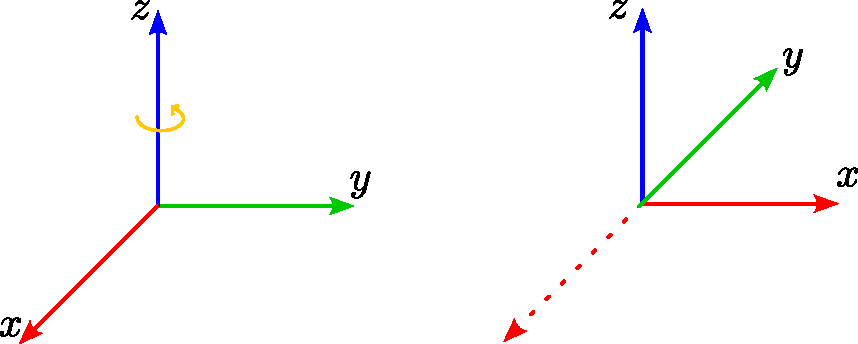
\includegraphics[width=\columnwidth]{./images/3d_rotation_example.pdf}
    \end{minipage}
    \hspace{1em}
    \begin{minipage}{0.70\linewidth}
        \small
        \begin{equation*}
            {\displaystyle R_{z}\left(\frac{\pi}{2}\right){\begin{bmatrix}1\\0\\0\\\end{bmatrix}}={\begin{bmatrix}\cos \frac{\pi}{2}&-\sin \frac{\pi}{2}&0\\\sin \frac{\pi}{2}&\quad \cos \frac{\pi}{2}&0\\0&0&1\\\end{bmatrix}}{\begin{bmatrix}1\\0\\0\\\end{bmatrix}}={\begin{bmatrix}0&-1&0\\1&0&0\\0&0&1\\\end{bmatrix}}{\begin{bmatrix}1\\0\\0\\\end{bmatrix}}={\begin{bmatrix}0\\1\\0\\\end{bmatrix}}}
        \end{equation*}
    \end{minipage}
\end{center}

\end{frame}

\begin{frame}
    \frametitle{Right-hand rule}
    En Robótica la disposición de los ejes de coordenadas y el sentido de rotación de los mismos está dado por la regla de la mano derecha (Right-hand rule).
    
    \begin{figure}[!h]
        \centering
        \subfloat[]
        {
            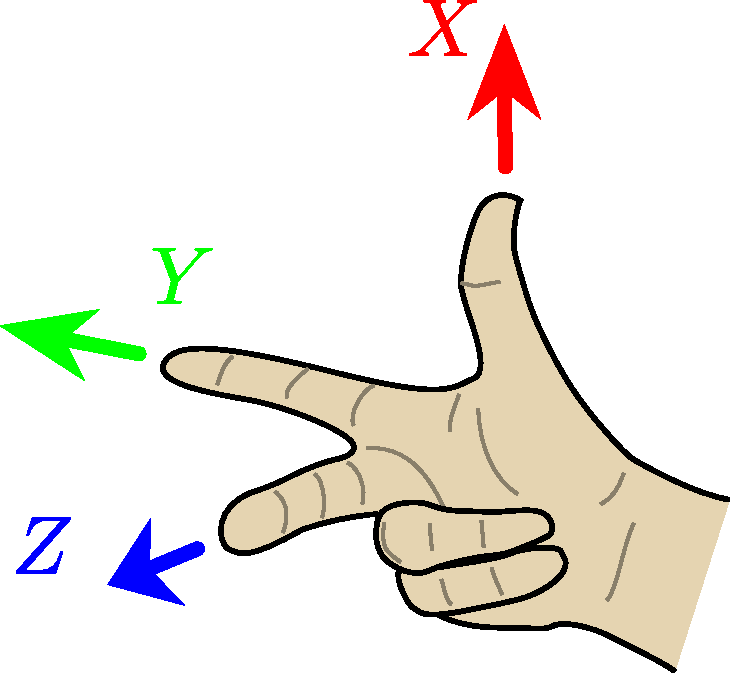
\includegraphics[width=0.4\columnwidth]{./images/right_hand_rule.pdf}
        }\hspace{1cm}
        \subfloat[]
        {
            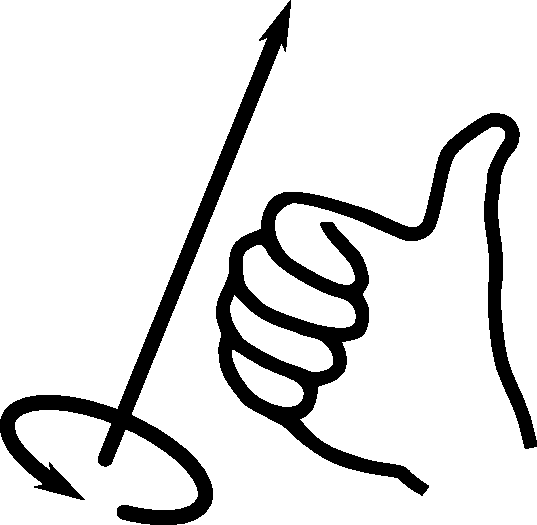
\includegraphics[width=0.4\columnwidth]{./images/right_hand_rule_positive_rotation.pdf}
        }
    \end{figure}
\end{frame}

\begin{frame}
    \frametitle{Roll Pitch Yaw }
    
    \begin{figure}[!h]
        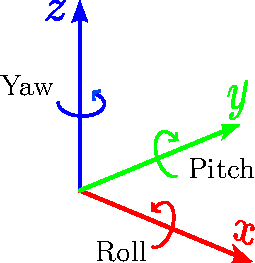
\includegraphics[width=0.4\columnwidth]{./images/roll_pitch_yaw.pdf}
    \end{figure}
\end{frame}

\begin{frame}
    \frametitle{Left-hand vs Right-hand rule}
    
    \only<1>{
        \begin{figure}
            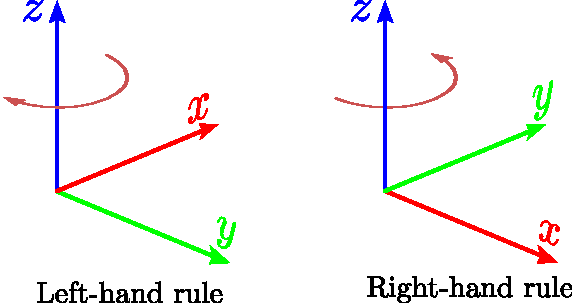
\includegraphics[width=0.9\columnwidth]{./images/left_right_hand_rule.pdf}
        \end{figure}
    }
    \only<2>{
        \begin{figure}
            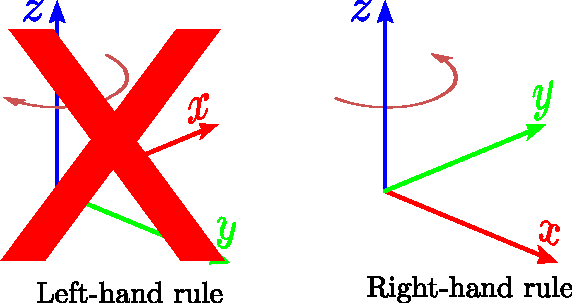
\includegraphics[width=0.9\columnwidth]{./images/left_right_hand_rule_cross.pdf}
        \end{figure}
    }
\end{frame}

\begin{frame}
    \frametitle{Rotaciones Generales 3D: Rotaciones Extrínsecas vs Rotaciones Intrínsecas}
    \scriptsize
    \begin{block}{Rotación Intrínseca}
    Describe una rotación en relación con el sistema de coordenadas local del objeto. Los ejes del objeto pueden cambiar durante la rotación. La Rotación final se construye Posmultiplicación: $R = R_{x}(\alpha) \, R_{y}(\beta) \, R_{z}(\gamma)$.
    \end{block}

    \begin{center}
        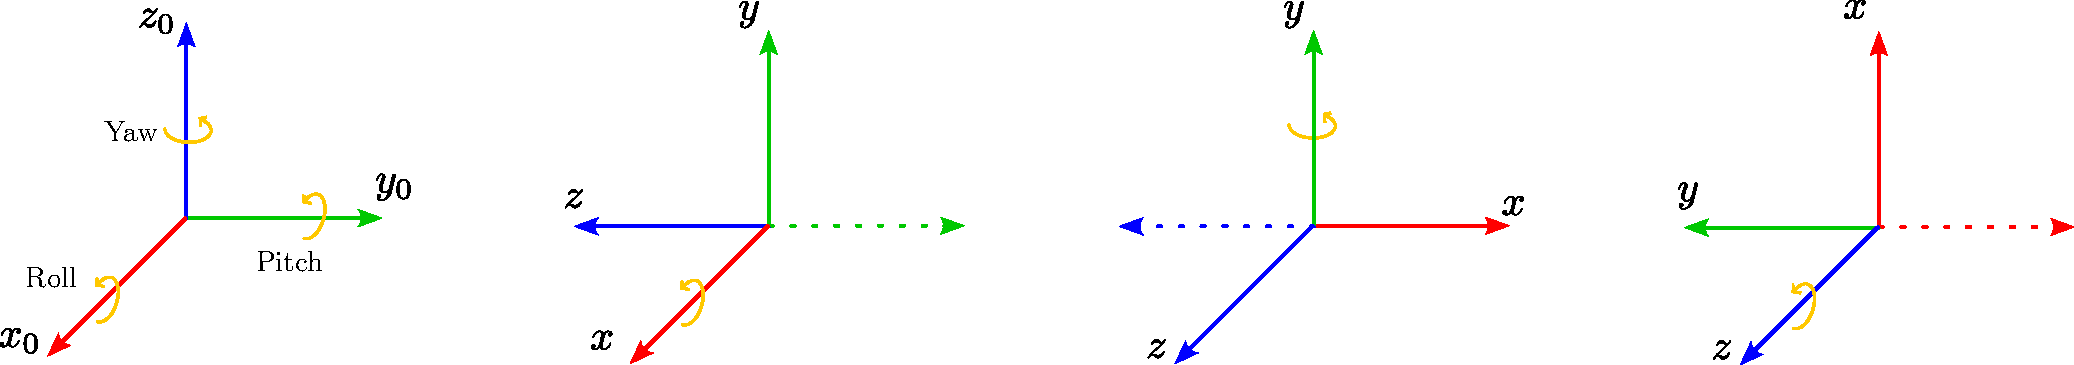
\includegraphics[width=0.7\columnwidth]{./images/intrinsic_rotation.pdf}
    \end{center}

    \begin{block}{Rotación Extrínseca}
        Describe una rotación en relación con un sistema de coordenadas global fijo en el espacio. El sistema de referencia es externo al objeto que está siendo rotado. La Rotación final se construye Premultiplicación: $R = R_{z}(\gamma) \, R_{y}(\beta) \, R_{x}(\alpha)$.
    \end{block}
    
    \begin{center}
        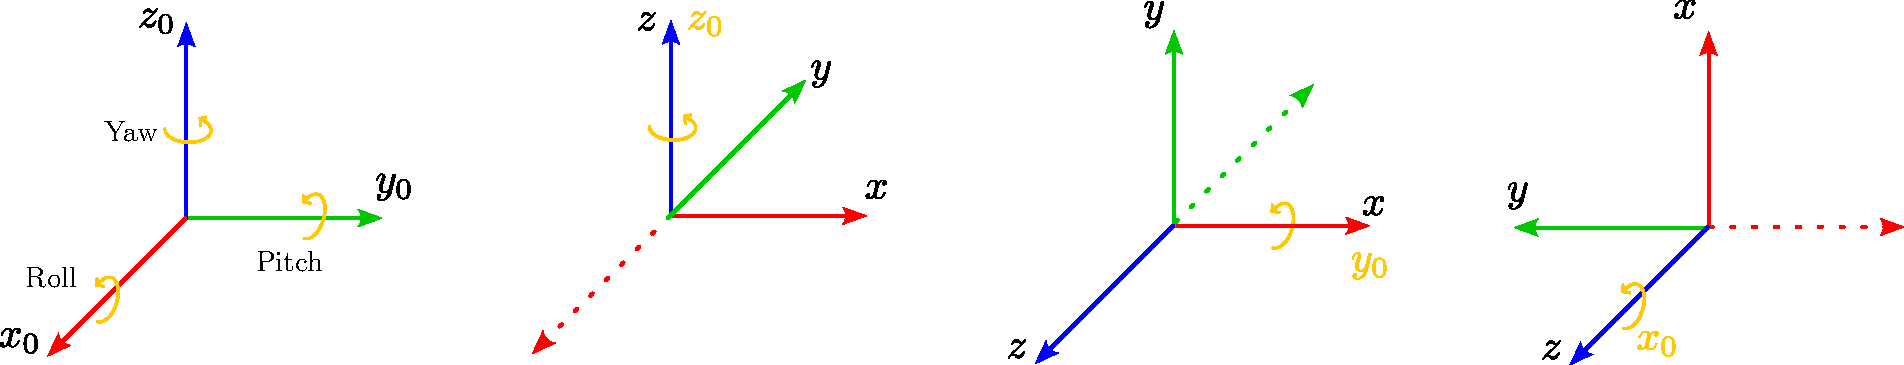
\includegraphics[width=0.7\columnwidth]{./images/extrinsic_rotation.pdf}
    \end{center}
        
    
    \note{Copiar slides donde se muestra que las rotaciones intrínsecas son equivalentes a las rotaciones extrínsecas: https://www.youtube.com/watch?v=icczqt73B7o}
    
\end{frame}

\begin{frame}
    \frametitle{Ángulos de Euler}
    \scriptsize
    \note{Euler se pruncia oiler.}

    \note{buen material:
        https://www.youtube.com/watch?v=d5sGRhjMXbY
        https://www.youtube.com/watch?v=geaUKjEYHtM
    }

    
    Una rotación de un de referencia a otro se puede obtener mediante la multiplicación de varias rotaciones.
    
    \begin{block}{Ángulos de Euler}
        Se denomina Ángulos de Euler a los ángulos $\alpha$, $\beta$ y $\gamma$ cuando estos deben ser aplicados utilizando el siguiente orden: $zxz$, $yxy$, $xyx$, $zyz$, $yzy$ y $xzx$. Los ángulos de Euler se aplican sobre el sistema de coordenadas local del objeto (Rotaciones intrínsecas).
    \end{block}
   
    Ejemplo de aplicación de Ángulos de Euler $\alpha$, $\beta$ y $\gamma$ utilizando la combinación $zxz$:
   \begin{figure}[!h]
           \centering
           \subfloat[$R = R_{x}(\alpha) \, R_{x}(\beta) \, R_{z}(\gamma)$]
           {
               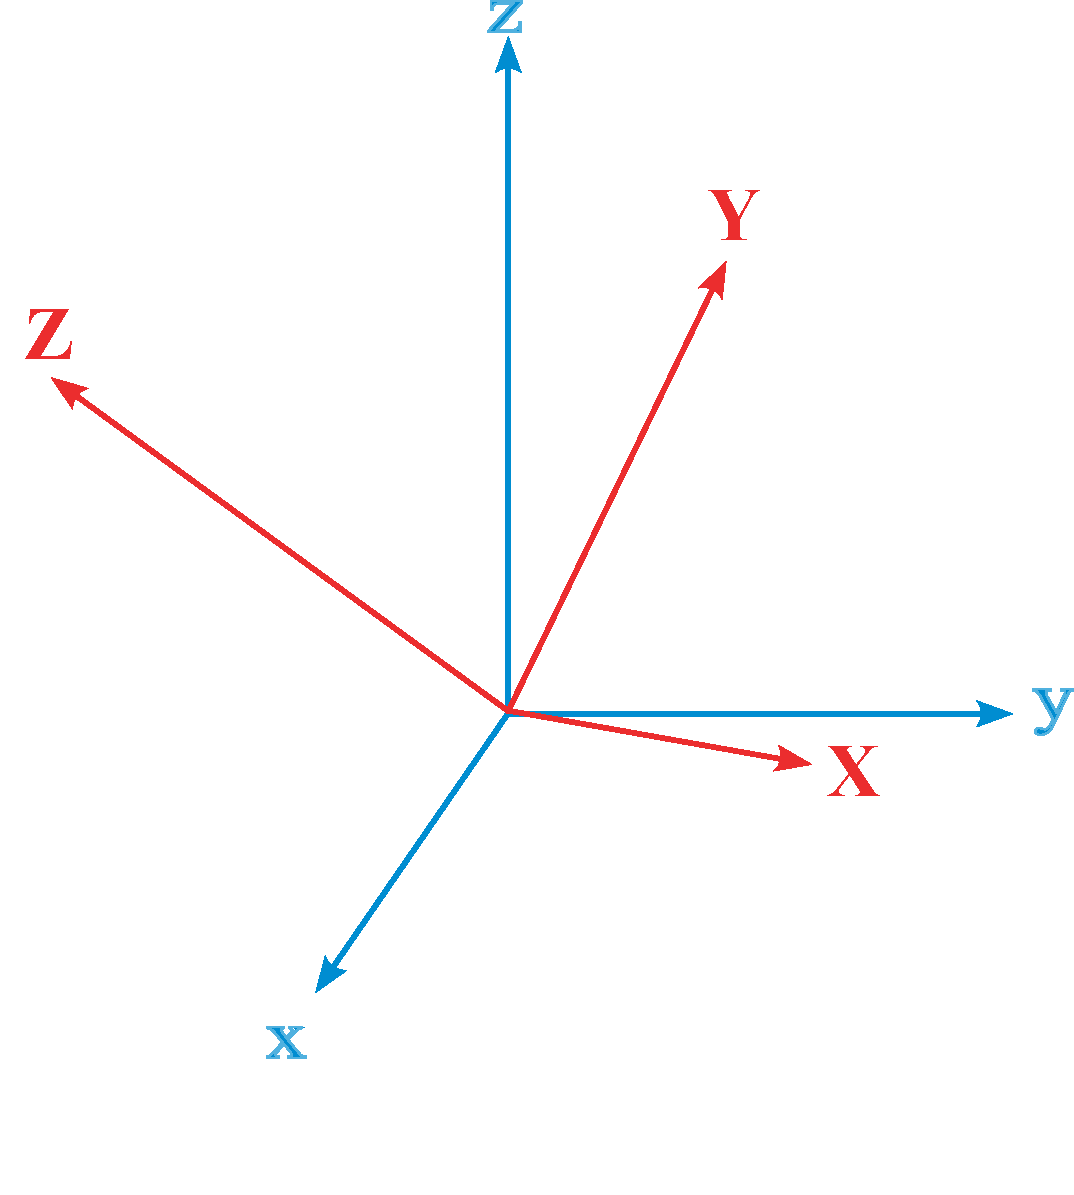
\includegraphics[width=0.23\columnwidth]{./images/euler_angles_initial.pdf}
           }
           \subfloat[$R_{z}(\alpha)$]
           {
               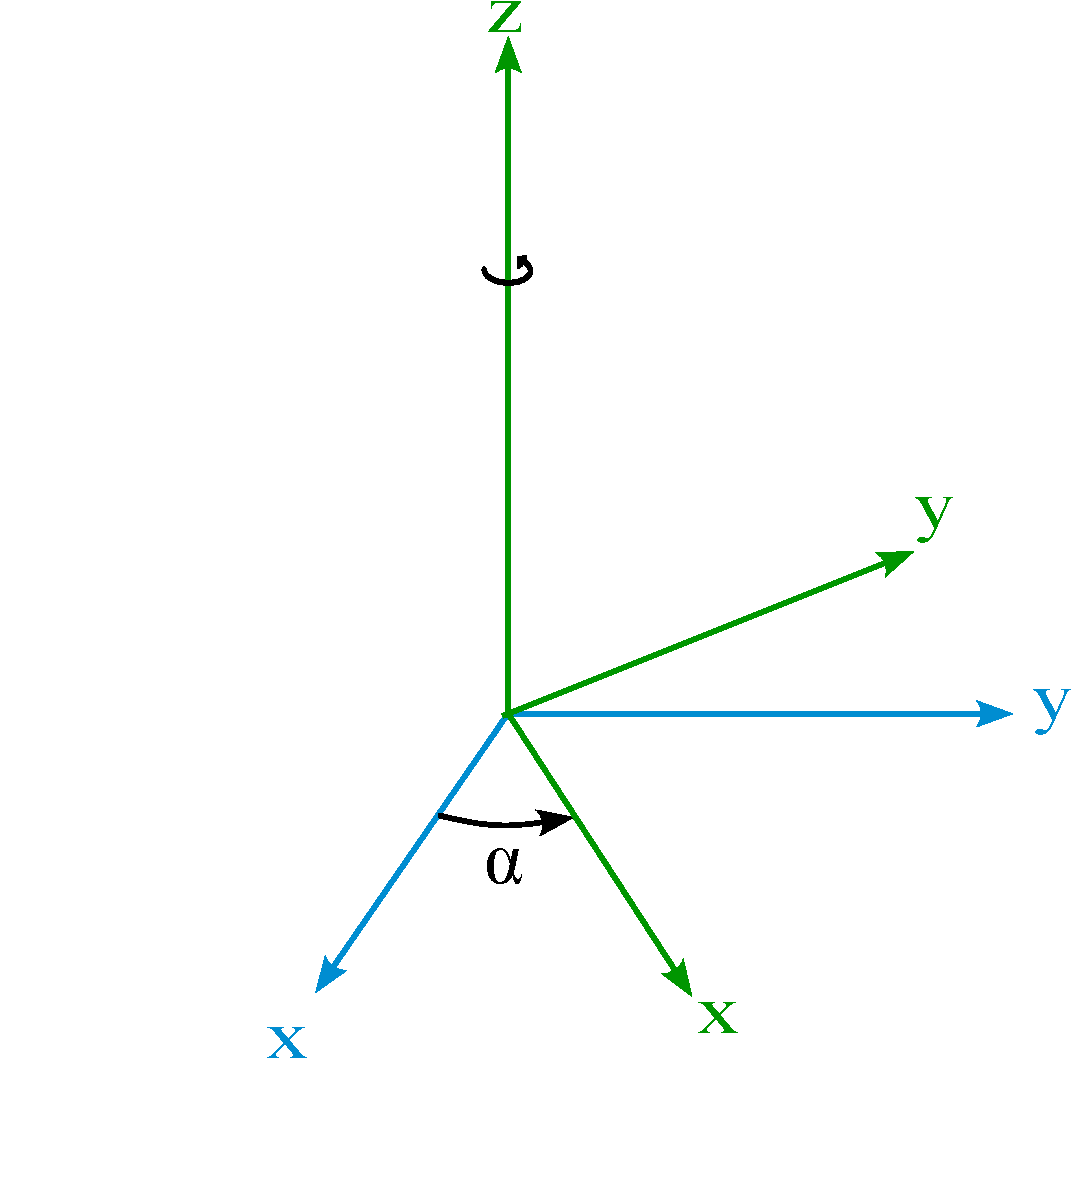
\includegraphics[width=0.23\columnwidth]{./images/euler_angles_alpha_rotation.pdf}
           }
           \subfloat[$R_{x}(\beta)$]
           {
               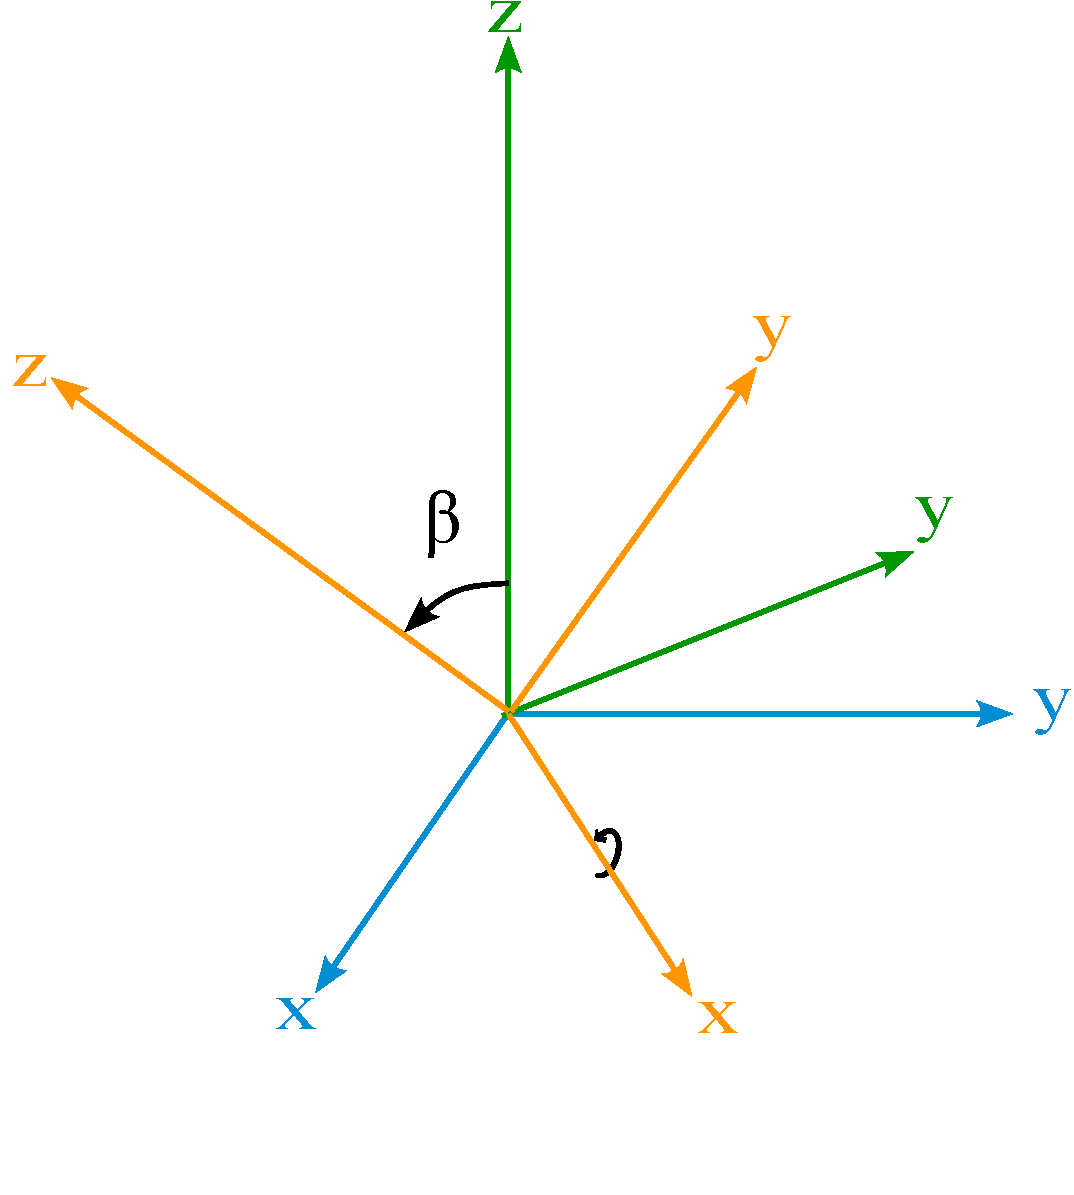
\includegraphics[width=0.23\columnwidth]{./images/euler_angles_beta_rotation.pdf}
           }
           \subfloat[$R_{z}(\gamma)$]
           {
               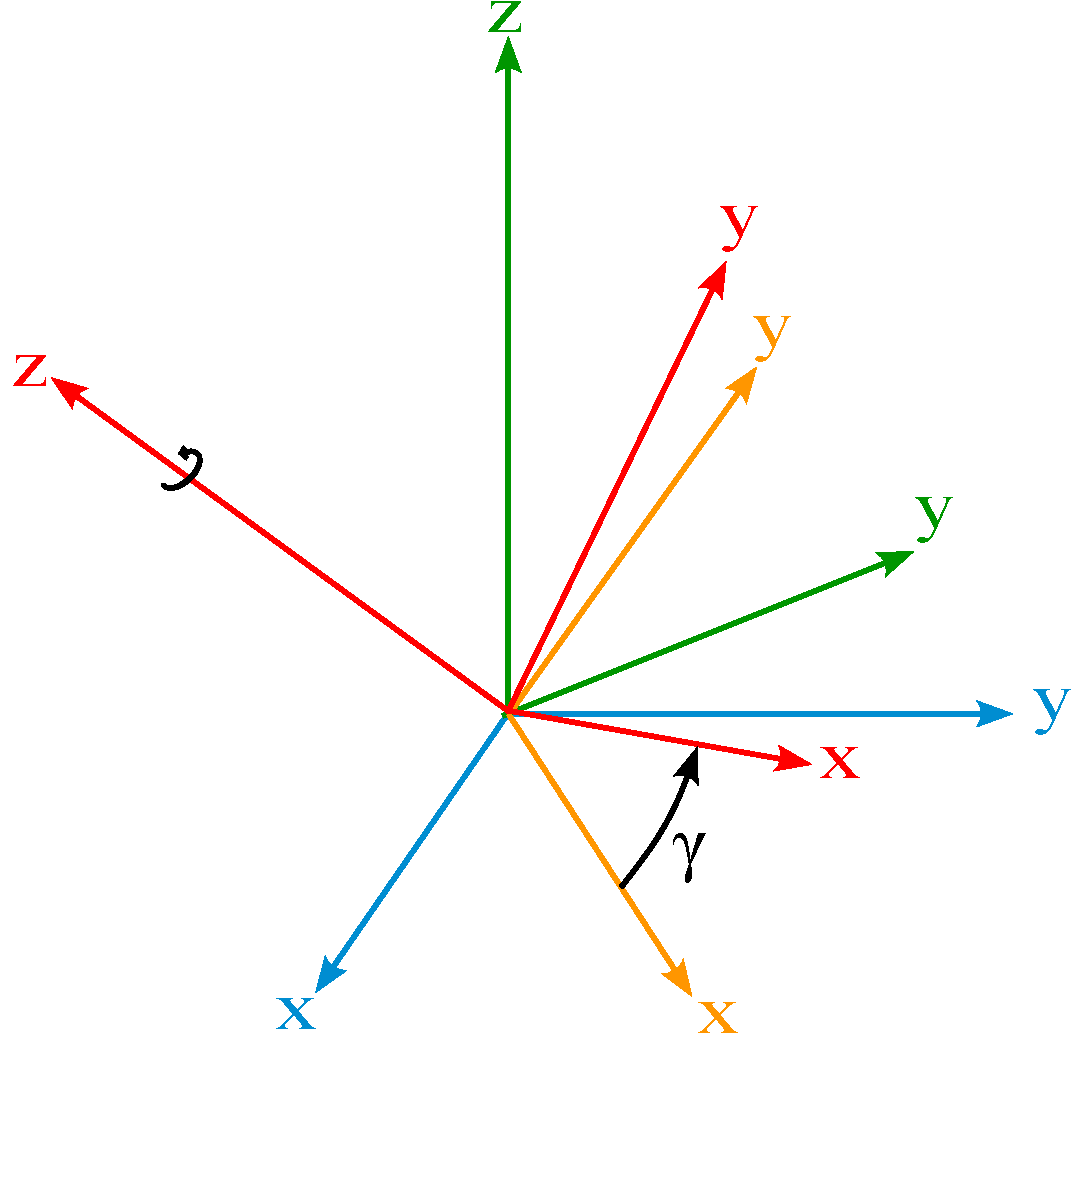
\includegraphics[width=0.23\columnwidth]{./images/euler_angles_gamma_rotation.pdf}
           }
    \end{figure}
\end{frame}


\begin{frame}
    \frametitle{Ángulos de Tait-Bryann}
    \small
    \begin{block}{Ángulos de Tait-Bryann}
        Combinaciones de giros con Ángulos de Tait-Bryann (o ángulos de navegación): $xyz$ $xzy$, $yxz$, $yzx$, $zxy$ y $zyx$. Los ángulos Tait-Bryann se usan normalmente para definir la orientación de aeronaves, satélites o embarcaciones. Los ángulos Tait-Bryann se aplican utilizando un sistema de coordenadas fijo (Rotaciones extrínsecas).
    \end{block}
    
    \begin{block}{Ángulos de Roll-Pitch-Yaw}
        Específicamente, la combinación $zyx$ de Ángulos de Tait-Bryann se denomina $Roll$, $Pitch$ y $Yaw$.
    \end{block}
    
    Matríz de Rotación resultante utilizando ángulos Roll-Pitch-Yaw:
    \scriptsize
    \begin{align*}
        R = R_{z}(\gamma) \, R_{y}(\beta) \, R_{x}(\alpha) &=
        \overset {\text{Yaw}}{
        \begin{bmatrix}
            \cos \gamma & -\sin \gamma & 0\\
            \sin \gamma & \cos \gamma &0\\
            0 & 0 & 1\\
        \end{bmatrix}}
        \overset {\text{Pitch}}{
        \begin{bmatrix}
            \cos \beta &0&\sin \beta\\
            0 & 1 & 0\\
            -\sin \beta &0&\cos \beta\\
        \end{bmatrix}}
        \overset {\text{Roll}}{
        \begin{bmatrix}
            1 & 0 & 0 \\
            0 & \cos \alpha & -\sin \alpha \\
            0& \sin \alpha & \cos \alpha \\
        \end{bmatrix}}\\
        &=
        \begin{bmatrix}
            \cos \beta \cos \gamma & \sin \alpha \sin \beta \cos \gamma - \cos \alpha \sin \gamma & \cos \alpha \sin \beta \cos \gamma + \sin \alpha \sin \gamma \\
            \cos \beta \sin \gamma & \sin \alpha \sin \beta \sin \gamma + \cos \alpha \cos \gamma & \cos \alpha \sin \beta \sin \gamma - \sin \alpha \cos \gamma \\
            -\sin \beta & \sin \alpha \cos \beta & \cos \alpha \cos \beta
        \end{bmatrix}
    \end{align*}
    
    \note{fuente: https://www.youtube.com/watch?v=oaq4Z4rbKkA}
    
    \note{fuente: https://www.youtube.com/watch?v=icczqt73B7o}
    
    \note{Davenport demostró que se puede lograr descomponer cualquier orientación mediante la sucesión de tres rotaciones elementales utilizando ejes no ortogonales. Las rotaciones elementales pueden darse respecto a los ejes del sistema de coordenadas fijo (rotaciones extrínsecas) o sobre los ejes de un sistema de coordenadas giratorio, que inicialmente se alinea con el sistema de ejes fijo y modifica su orientación después de cada rotación elemental (rotaciones intrínsecas).
        
        Según el teorema de Davenport, es posible una descomposición única si y solo si el segundo eje es perpendicular a los otros dos ejes. Por lo tanto, los ejes 1 y 3 deben estar en el plano ortogonal al eje 2.
        
        En consecuencia, las descomposiciones de las rotaciones encadenadas de Euler y de las rotaciones encadenadas de Tait-Bryan son casos particulares de esta configuración general. El caso de Tait-Bryan aparece cuando los ejes 1 y 3 son perpendiculares, y el caso de Euler aparece cuando se superponen.
    }
    
\end{frame}

\begin{frame}
    \frametitle{Ángulos de Euler y Gimbal Lock (Bloqueo de Cardan)}
    \scriptsize

    Cuando representamos una Rotación con ángulos de Euler se puede producir una situación similar al Bloqueo de Cardan (\emph{Gimbal Lock}).    
    
    \begin{center}
        \movie[autostart,loop,poster]{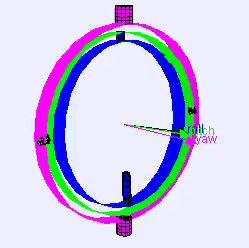
\includegraphics[width=0.2\textwidth]{./images/gimbal_rotation.png}}{./videos/gimbal_rotation.mp4}\hspace{1em}
        \movie[autostart,loop,poster]{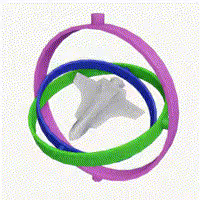
\includegraphics[width=0.2\textwidth]{./images/gimbal_lock_video.png}}{./videos/gimbal_lock.mp4}
    \end{center}
    
    \note{La palabra ``bloqueo'' puede ser confusa: ninguno de los cardanes (\emph{gimbals}) está bloqueado. Los tres pueden todavía moverse libremente sobre sus ejes de suspensión respectivos. Sin embargo, debido a la orientación paralela de los ejes de dos de los cardanes, existe un eje sobre el que ninguno de los cardanes puede girar.}
    
    \begin{itemize}
        \item Pérdida de un grado de libertad cuando dos de los tres ejes de giro se colocan en paralelo.
        \item Existe un eje sobre el que no se puede girar. En la práctica, por ejemplo, puede hacer que un brazo robótica no pueda realizar cierto giro. Solución: \emph{wrist flip}.
    \end{itemize}
    
    \note{En el caso de los ángulos de Euler, lo que sucede es que dos de los tres ángulos describen un mismo giro. El Gimbal Lock ocurre específicamente en los ángulos de Euler cuando los giros se aplican en un orden particular, generalmente cuando el ángulo de Pitch se acerca a 90 grados.}
    
    Tool Online para mostrar Gimbal Lock: \url{https://danceswithcode.net/engineeringnotes/rotations_in_3d/demo3D/rotations_in_3d_tool.html}
    

    \note{El Gimbal Lock ocurre cuando dos de los ejes de rotación se vuelven paralelos entre sí. Esto elimina un grado de libertad y limita la capacidad del objeto para rotar libremente en todas las direcciones. En términos más simples, el objeto queda atrapado en un estado en el que solo puede rotar alrededor de dos ejes en lugar de tres. Esto puede dificultar el control y la representación precisa de la orientación del objeto.}
      
    Los ángulos de Euler proporcionan una descripción numérica de cualquier rotación en el espacio tridimensional usando tres reales $\alpha$, $\beta$ y $\gamma$. Pero no sólo no es esta descripción única sino que además existen puntos sobre los que \textbf{no todo cambio en el espacio de rotaciones puede ser expresado como un cambio en el espacio de los ángulos de Euler}.
    
    El Gimbal Lock generó un incidente en el Apolo 11.
    
    \note{Problema del Apollo 11 con Gimbal Lock: https://history.nasa.gov/alsj/gimbals.html}

    \note{https://youtu.be/Mm8tzzfy1Uw}
    \note{https://youtu.be/oaq4Z4rbKkA}
    \note{Gimbal-Lock Video explanation: https://youtu.be/-WXfEPg8eMM}
\end{frame}

\begin{frame}
    \frametitle{Propiedades de matrices Rotación}
    \small
    \begin{itemize}
        \item $R^{\mathsf {T}}=R^{-1}$ Matriz ortogonal
        \item $\det R = \pm 1$ (esto implica que la longitud del vector no cambia luego de la rotación)
        \item $R \in SO(3)$ entonces $\rotationCoord{A}{C} = \rotationCoord{A}{B} \rotationCoord{B}{C}$ y $\rotationCoord{A}{B} = \rotationCoord{B}{A}^{-1}$
        \item \TODO{Agregar imagen y explicar mejor: Los vectores columnas de la matriz de Rotación muestran donde se encuentran posicionados los ejes x, y y z luego de aplicar la rotación}
    \end{itemize}

    Determinar el ángulo de una matriz de rotación utilizando la traza de la matriz (la suma de los elementos de la diagonal del matriz).
    \begin{equation*}
        {\displaystyle \operatorname {tr} (R)=1+2\cos \theta ,}
    \end{equation*}

    \begin{equation*}
        {\displaystyle |\theta |=\arccos \left({\frac {\operatorname {tr} (R)-1}{2}}\right).}
    \end{equation*}

\end{frame}

\begin{frame}
    \frametitle{Rotación representada con Axis-angle}
    La notación axial-angular es equivalente al más conciso vector de rotación, también llamado vector de Euler. En este caso, tanto el eje de rotación como el ángulo están representados por un vector codireccional con el eje de rotación cuyo módulo (longitud) coincide con el ángulo de rotación $\theta$,
    \begin{center}
        \begin{minipage}{0.38\linewidth}
            \small
            \begin{equation*}
                {\displaystyle {\boldsymbol {\theta }}=\theta \mathbf {e} \,.}
            \end{equation*}
            \begin{equation*}
                {\displaystyle (\mathrm {eje} ,\mathrm {\text{ángulo}} )=\left({\begin{bmatrix}e_{x}\\e_{y}\\e_{z}\end{bmatrix}},\theta \right)}
            \end{equation*}
        \end{minipage}
        \hspace{1em}
        \begin{minipage}{0.38\linewidth}
            \centering
            \begin{figure}
               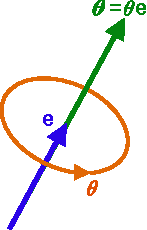
\includegraphics[width=0.3\columnwidth]{images/axis_angle_vector.pdf}
            \end{figure}
        \end{minipage}
    \end{center}

    Ejemplo un vector de rotación con una magnitud de $\dfrac{\pi}{2}$ apuntando en la dirección $z$:
    \begin{equation*}
        {\displaystyle {\left({\begin{bmatrix}0\\0\\1\end{bmatrix}},{\frac {\pi }{2}}\right) = \begin{bmatrix}0\\0\\{\frac {\pi }{2}}\end{bmatrix}}.}
    \end{equation*}

    \note{The representation is very intuitive, but for actually applying the rotation, another representation is required, such as a quaternion or rotation matrix.}

\end{frame}

\begin{frame}
    \frametitle{Quaternions}
    Los cuaterniones es una generalización de números complejos con tres números imaginarios (i, j y k). Es un número complejo de cuatro dimensiones que se puede utilizar para representar la orientación de un cuerpo rígido o un marco de coordenadas en un espacio tridimensional. La definición general de un cuaternión viene dada por:
    %
    \begin{equation*}
        q = w + q_x i + q_y j + q_z k = \begin{bmatrix} q_w & q_x & q_y & q_z\end{bmatrix}
    \end{equation*}
\end{frame}

\begin{frame}
    \frametitle{Quaternions}
    \scriptsize
    \begin{center}
        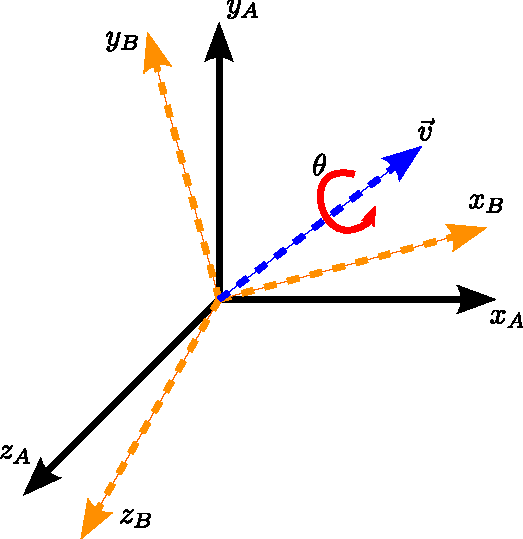
\includegraphics[width=0.2\columnwidth]{./images/quaternion.pdf}
    \end{center}

    Los cuaterniones representan una transformación de rotación en 3D. Por lo tanto, la forma más fácil de representar un cuaternión es imaginar la rotación de un ángulo dado alrededor de un vector dado. La figura ilustra la rotación del ángulo $\theta$ alrededor del vector $\vec{v} = [v_{x} v_{y} v_{z}]$. El cuaternión asociado a esta rotación está dado por:
    %
    \begin{align*}
        q &= \begin{bmatrix} q_w & q_x & q_y & q_z\end{bmatrix}\\
        q &= \begin{bmatrix}
            \cos \frac{\theta}{2} & v_{x} \sin \frac{\theta}{2} & v_{y} \sin \frac{\theta}{2} & v_{z}\sin \frac{\theta}{2}
        \end{bmatrix}
    \end{align*}

    Ventajas:
    \begin{itemize}
        \item Componer rotaciones es más rápido y numéricamente más estable
        \item Extraer el ángulo y el eje de rotación es más simple
        \item Interpolar dos rotaciones es más directo (utilizando la función $slerp()$)
        \item Los cuaterniones no sufren de \emph{Gimbal Lock} como los ángulos de Euler.
    \end{itemize}

\end{frame}
